Радиопередающий модуль FS1000A представляет собой низкобюджетное устройство передачи радиосообщений (рисунок~\ref{fig:fs1000a}). Спецификация FS1000A представлена ниже~\cite{fs1000a:specs}:

\begin{figure}[ht]
    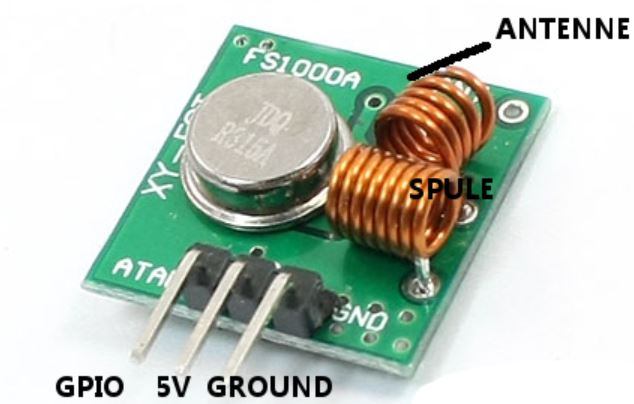
\includegraphics[width=.3\linewidth]{Figures/fs1000a.jpg}
    \caption{Радиопередатчик FS1000A}
    \label{fig:fs1000a}
\end{figure}

\begin{longtable}[c]{|c|c|}
    \caption{Спецификация модуля FS1000A}
    \label{tab:specs}\\
    \hline
    \textbf{Параметр} & \textbf{Значение}\\
    \hline
    \endfirsthead
    \hline
    \textbf{Параметр} & \textbf{Значение}\\
    \hline
    \endhead
        Входное напряжение & 2.5 -- 12 В\\
        \hline
        Тип модуляции & Амплитудная\\
        \hline
        Максимальная скорость передачи данных & 9.6 Кбит/с\\
        \hline
\end{longtable}

Скорость передачи данных в данном случае говорит, что за одну секунду можно передать блок данных размером в $\frac{9.6}{8} = 1.2$ Кб, или 9600 бит. Другими словами, если отправлять пачку длиной в 1 бит как полноценное сообщение с передатчика на приёмник, максимально доступной частотой для нас будет 9.6 КГц. Однако для надёжной передачи сообщения необходимо \textbf{как минимум} 3 бита: синхронизирующий бит, бит данных и ещё один бит данных, представляющий собой инверсию данных для подтверждения подлинности. Естественно, чем больше битов в синхронизирующем сообщении и в самом сообщении, тем надёжнее будет посылка.

Если взглянуть в справочник по передачи данных на физическом уровне (через UART), можно также заметить, что стандартное время передачи одного символа (12 бит) на скорости 9600 бит/с не превышает 1.25 мсек (рисунок~\ref{fig:mits})~\cite{mits:fx}:

\begin{figure}[ht]
    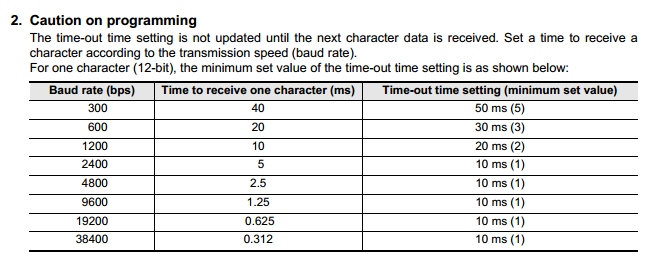
\includegraphics[width=1\linewidth]{Figures/mits.png}
    \caption{Скорость передачи данных (PLC Data Communication Manual)}
    \label{fig:mits}
\end{figure}
